\documentclass[a4paper]{article} 
\addtolength{\hoffset}{-2.25cm}
\addtolength{\textwidth}{4.5cm}
\addtolength{\voffset}{-3.25cm}
\addtolength{\textheight}{5cm}
\setlength{\parskip}{0pt}
\setlength{\parindent}{0in}

%----------------------------------------------------------------------------------------
%	PACKAGES AND OTHER DOCUMENT CONFIGURATIONS
%----------------------------------------------------------------------------------------

\usepackage{blindtext} % Package to generate dummy text
\usepackage{tikz}
\usetikzlibrary{positioning, arrows.meta}

\usepackage{charter} % Use the Charter font
\usepackage[utf8]{inputenc} % Use UTF-8 encoding
\usepackage{microtype} % Slightly tweak font spacing for aesthetics
\usepackage[english]{babel} % Language hyphenation and typographical rules
\usepackage{amsthm, amsmath, amssymb} % Mathematical typesetting
\usepackage{algorithm}
\usepackage{algorithmic}
\usepackage{float} % Improved interface for floating objects
\usepackage[final, colorlinks = true, 
            linkcolor = black, 
            citecolor = black]{hyperref} % For hyperlinks in the PDF
\usepackage{graphicx, multicol} % Enhanced support for graphics
\usepackage{xcolor} % Driver-independent color extensions
\usepackage{marvosym, wasysym} % More symbols
\usepackage{rotating} % Rotation tools
\usepackage{censor} % Facilities for controlling restricted text
\usepackage{listings, style/lstlisting} % Environment for non-formatted code, !uses style file!
% \usepackage{pseudocode} % Environment for specifying algorithms in a natural way
\usepackage{style/avm} % Environment for f-structures, !uses style file!
\usepackage{booktabs} % Enhances quality of tables
\usepackage{tikz-qtree} % Easy tree drawing tool
\tikzset{every tree node/.style={align=center,anchor=north},
         level distance=2cm} % Configuration for q-trees
\usepackage{style/btree} % Configuration for b-trees and b+-trees, !uses style file!
\usepackage[backend=biber,style=numeric,
            sorting=nyt]{biblatex} % Complete reimplementation of bibliographic facilities
\addbibresource{ecl.bib}
\usepackage{csquotes} % Context sensitive quotation facilities
\usepackage[explicit]{titlesec}
\titleformat{\section}{\normalfont\Large\bfseries}{}{0em}{#1\ \thesection}
\renewcommand{\thesubsection}{\thesection.\alph{subsection}}
\usepackage[yyyymmdd]{datetime} % Uses YEAR-MONTH-DAY format for dates
\renewcommand{\dateseparator}{-} % Sets dateseparator to '-'
\usepackage{fancyhdr} % Headers and footers
\pagestyle{fancy} % All pages have headers and footers
\fancyhead{}\renewcommand{\headrulewidth}{0pt} % Blank out the default header
\fancyfoot[L]{} % Custom footer text
\fancyfoot[C]{} % Custom footer text
\fancyfoot[R]{\thepage} % Custom footer text
\newcommand{\note}[1]{\marginpar{\scriptsize \textcolor{red}{#1}}} % Enables comments in red on margin
% -------------------Added by meeeeeeeee,Prateek
\usepackage{xcolor}
\usepackage{subcaption}

% \definecolor{codegreen}{rgb}{0,0.6,0}
% \definecolor{codegray}{rgb}{0.5,0.5,0.5}
% \definecolor{codepurple}{rgb}{0.58,0,0.82}
% \definecolor{backcolour}{rgb}{0.95,0.95,0.92}

% \lstdefinestyle{mystyle}{
%     backgroundcolor=\color{backcolour},   
%     commentstyle=\color{codegreen},
%     keywordstyle=\color{magenta},
%     numberstyle=\tiny\color{codegray},
%     stringstyle=\color{codepurple},
%     basicstyle=\ttfamily\footnotesize,
%     breakatwhitespace=false,         
%     breaklines=true,                 
%     captionpos=b,                    
%     keepspaces=true,                 
%     numbers=left,                    
%     numbersep=5pt,                  
%     showspaces=false,                
%     showstringspaces=false,
%     showtabs=false,                  
%     tabsize=2
% }

% \lstset{style=mystyle}
\DeclareMathOperator*{\argmax}{arg\,max}
\DeclareMathOperator*{\argmin}{arg\,min}
%----------------------------------------------------------------------------------------



\begin{document}

%-------------------------------
%	TITLE SECTION
%-------------------------------

\fancyhead[C]{}
\hrule \medskip % Upper rule
\begin{minipage}{0.295\textwidth} 
\raggedright
\footnotesize
Saksham, Deeksha, Sharvanee  \hfill\\   
22B1003, 22B0988, 22B0943\hfill\\
Bayesian Bunch
\end{minipage}
\begin{minipage}{0.4\textwidth} 
\centering 
\large 
Undirected Graphical Models\\ 
\normalsize 
Advanced Machine Learning (Spring '25)\\ 
\end{minipage}
\begin{minipage}{0.295\textwidth} 
\raggedleft
\today\hfill\\
\end{minipage}
\medskip\hrule 
\bigskip
\section{Class Query}
Based on one of the questions raised in class, ma'am clarified that:

\[X \perp\!\!\!\perp \{Y_1, \dots, Y_k\} \mid Z\implies (X \perp\!\!\!\perp Y_1 | Z) \dots (X \perp\!\!\!\perp Y_k | Z)\]
However, the reverse might not be true. So, the following does not hold:

\[(X \perp\!\!\!\perp Y_1 | Z)  \dots  (X \perp\!\!\!\perp Y_k | Z) \implies X \perp\!\!\!\perp \{Y_1, \dots, Y_k\} \mid Z\]


\section{Undirected Graphical Models}
In this model, the underlying graph which represents the probability distribution is undirected. Such a model is useful when the variables interact symmetrically, and there is no natural parent-child relationship. Some of the natural examples, which represent such a scenario include friends on a social media platform, atoms in a crystal, labelling pixels in an image, etc.

In an undirected graphical model, we define potentials over arbitrary cliques of the graph $G$. (Cliques are subsets of nodes of a graph which are fully connected, i.e they are complete subgraphs of a graph.) The potentials are denoted by $\psi_C(y_C)$. The first subscript $C$ denotes the clique in consideration, and $y_C$ denotes the assignment to the variables in the clique.

Potentials can take arbitrary non-negative values, however they cannot be considered equivalent to probabilities. 

Here is how we define the joint distribution in an undirected graphical model:

\[
Pr(y_1, \dots, y_n) = \frac{1}{Z} \prod_{C \in \mathcal{C}} \psi_C(y_C)
\]

where $\mathcal{C}$ is the set of all cliques in the graph, and $Z$ is the normalizing constant, which ensures that the sum of all probabilities is equal to 1. For the numerator, what we essentially do is for that particular assignment of variables, we take a product over all the cliques in the graph, and multiply the potentials for that assignment.

Here is how we define $Z$:

\[
Z = \sum_{y_1} \dots \sum_{y_n} \prod_{C \in \mathcal{C}} \psi_C(y_C)
\]

This expression of $Z$ is also called the partition function. For calculating $Z$, what we essentially do is to sum over all possible assignments of variables, and take a product over all the cliques in the graph, and multiply the potentials for that assignment. This ensures that the sum of all probabilities is equal to 1.


\subsection{Example}
\begin{minipage}{0.55\textwidth} 
    Consider the graph $G$ shown on the right. There are 9 binary variables $y_1, y_2, \dots, y_9$ (each can take only two values 0 or 1).  

    There are two types of cliques in this graph, one is the set of all edges, and the other is the set of all nodes. The potentials for the edges are denoted by $\psi_{ij}(y_i, y_j)$, and the potentials for the nodes are denoted by $\psi_i(y_i)$.

    The joint distribution for this graph can be written as:

    \[
    Pr(y_1, \dots, y_9) = \frac{1}{Z} \prod_{i=1}^{9} \psi_i(y_i) \prod_{(i,j) \in E} \psi_{ij}(y_i, y_j)
    \]

    where $E$ is the set of all edges in the graph.

\end{minipage}
\hfill 
\begin{minipage}{0.40\textwidth} 
    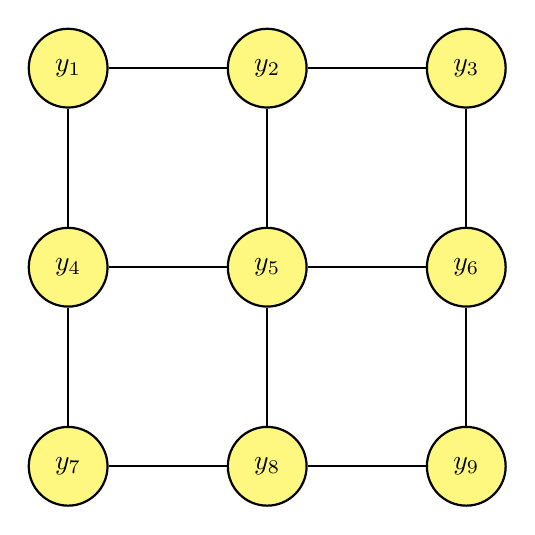
\begin{tikzpicture}[node distance=1.5cm and 1.5cm, thick, every node/.style={circle, draw, fill=yellow!50, minimum size=1cm}]
        \node (y1) {$y_1$};
        \node[right=of y1] (y2) {$y_2$};
        \node[right=of y2] (y3) {$y_3$};
        \node[below=of y1] (y4) {$y_4$};
        \node[right=of y4] (y5) {$y_5$};
        \node[right=of y5] (y6) {$y_6$};
        \node[below=of y4] (y7) {$y_7$};
        \node[right=of y7] (y8) {$y_8$};
        \node[right=of y8] (y9) {$y_9$};
        \draw (y1) -- (y2);
        \draw (y2) -- (y3);
        \draw (y1) -- (y4);
        \draw (y2) -- (y5);
        \draw (y3) -- (y6);
        \draw (y4) -- (y5);
        \draw (y5) -- (y6);
        \draw (y4) -- (y7);
        \draw (y5) -- (y8);
        \draw (y6) -- (y9);
        \draw (y7) -- (y8);
        \draw (y8) -- (y9);
    \end{tikzpicture}
\end{minipage}


For example, the value of $Pr(1, 0, \dots, 0)$ can be calculated as:

\[
Pr(1, 0, \dots, 0) = \frac{1}{Z} \begin{aligned}[t]
& \psi_1(1) \psi_2(0) \psi_3(0) \dots \psi_9(0) \psi_{12}(1, 0) \psi_{23}(0, 0) \psi_{14}(1, 0) \psi_{25}(0, 0) \\
& \psi_{36}(0, 0) \psi_{45}(0, 0) \psi_{56}(0, 0) \psi_{47}(0, 0) \psi_{58}(0, 0) \\
& \psi_{69}(0, 0) \psi_{78}(0, 0) \psi_{89}(0, 0)
\end{aligned}
\]

$Z$ can be calculated as follows:

\[
Z = \sum_{y_1} \dots \sum_{y_9} \begin{aligned}[t]
& \psi_1(y_1) \psi_2(y_2) \psi_3(y_3) \dots \psi_9(y_9) \psi_{12}(y_1, y_2) \psi_{23}(y_2, y_3) \psi_{14}(y_1, y_4) \psi_{25}(y_2, y_5) \\
& \psi_{36}(y_3, y_6) \psi_{45}(y_4, y_5) \psi_{56}(y_5, y_6) \psi_{47}(y_4, y_7) \psi_{58}(y_5, y_8) \\
& \psi_{69}(y_6, y_9) \psi_{78}(y_7, y_8) \psi_{89}(y_8, y_9) 
\end{aligned}
\]

In this case, we need to sum over 512 possible assignments of variables, which is computationally expensive.


Another example was given. It was a K3 (complete graph with 3 nodes). If we consider only one clique (the complete graph), then the joint distribution can be written as (an example):

\[
    P(y_1 = 0, y_2 = 1, y_3 = 1) = \frac{\psi_{123}(0, 1, 1)}{\psi_{123}(0, 0, 0) + \psi_{123}(0, 0, 1) + \dots + \psi_{123}(1, 1, 1)}
\]

Similarly, if we consider only the three edges as the cliques, then the joint distribution can be written as:

\[
    P(y_1 = 0, y_2 = 1, y_3 = 1) = \frac{\psi_{12}(0, 1) \psi_{23}(1, 1) \psi_{13}(0, 1)}{\psi_{12}(0, 0) \psi_{23}(0, 0) \psi_{13}(0, 0) + \dots + \psi_{12}(1, 1) \psi_{23}(1, 1) \psi_{13}(1, 1)}
\]

The types of cliques, on which we define potential depends on the real world clue which we have. 


Also, the number of parameters needed to define potential is exponential in the number of nodes in the clique. Therefore, computing $Z$ is tough and for certain graphs we exploit factorization to simplify.

In general, if $|C| = k$, and $y_i \in \{1, \dots, m\}$, then the number of potential scores we need to report will be $m^k$.


\section{Conditional Independencies in an Undirected Graphical Model}
Let $V = \{y_1, \dots, y_n\}$.

Let distribution $P$ be represented by an undirected graphical model $G$. If $Z$ separates $X$ and $Y$ in $G$, then $X \perp\!\!\!\perp Y | Z$ in $P$. The set of all such CIs are called Global-CI of the UGM (undirected graphical model).

\begin{minipage}{0.55\textwidth} 
    Example:
    \begin{enumerate}
        \item $y_1 \perp\!\!\!\perp y_3, y_5, y_6, y_7, y_8, y_9 | y_2, y_4$
        \item $y_1 \perp\!\!\!\perp y_3|y_2,y_4,y_5,y_6,y_7,y_8,y_9$ (the separator $Z$ need not be minimal)
        \item $y_1,y_2,y_3 \perp\!\!\!\perp y_7,y_8,y_9|y_4,y_5,y_6$
        \item $y_1 \perp\!\!\!\perp y_3|y_2,y_4$
    \end{enumerate}

    (Basically when we remove $Z$, $X$ and $Y$ should be disconnected in the graph.)

\end{minipage}
\hfill 
\begin{minipage}{0.40\textwidth} 
    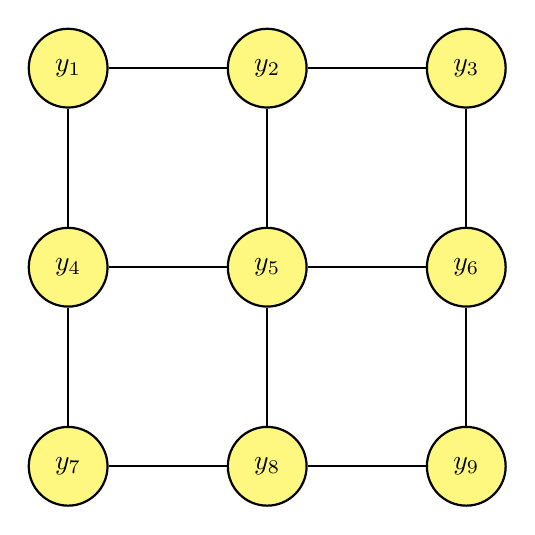
\begin{tikzpicture}[node distance=1.5cm and 1.5cm, thick, every node/.style={circle, draw, fill=yellow!50, minimum size=1cm}]
        \node (y1) {$y_1$};
        \node[right=of y1] (y2) {$y_2$};
        \node[right=of y2] (y3) {$y_3$};
        \node[below=of y1] (y4) {$y_4$};
        \node[right=of y4] (y5) {$y_5$};
        \node[right=of y5] (y6) {$y_6$};
        \node[below=of y4] (y7) {$y_7$};
        \node[right=of y7] (y8) {$y_8$};
        \node[right=of y8] (y9) {$y_9$};
        \draw (y1) -- (y2);
        \draw (y2) -- (y3);
        \draw (y1) -- (y4);
        \draw (y2) -- (y5);
        \draw (y3) -- (y6);
        \draw (y4) -- (y5);
        \draw (y5) -- (y6);
        \draw (y4) -- (y7);
        \draw (y5) -- (y8);
        \draw (y6) -- (y9);
        \draw (y7) -- (y8);
        \draw (y8) -- (y9);
    \end{tikzpicture}
\end{minipage}

\section{Factorization implies Global CI}
Here is the theorem:

Let $G$ be the undirected graph over $V = x_1, \dots, x_n$ nodes and $P(x_1, \dots, x_n)$ be a distribution. If $P$ is represented by $G$ that is, if it can be factorized as per the cliques of $G$, then $P$ will also satisfy the global-CIs of $G$.

Factorize($P, G$) $\implies$ Global-CI($P, G$)

\subsection{Example}

\begin{minipage}{0.55\textwidth} 
    One of the valid options to express $P$ is as follows:
    \[P(x_1, \dots, x_5) \propto \psi_{124}(x_1, x_2, x_4)\psi_{234}(x_2, x_3, x_4)\psi_{45}(x_4, x_5)\]

    Since, $P$ can be factorized as per the cliques of $G$, it will also satisfy the global-CIs of $G$. For example, $x_1 \perp\!\!\!\perp x_5 | x_2, x_3, x_4$ is a valid CI.
\end{minipage}
\hfill 
\begin{minipage}{0.40\textwidth} 
    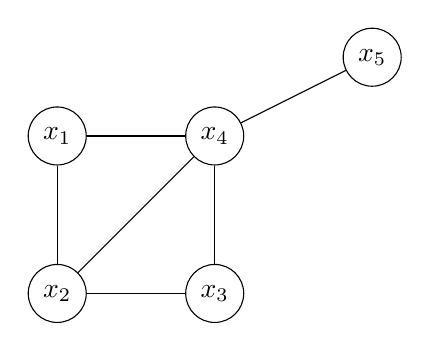
\begin{tikzpicture}[node distance=1.5cm, auto]

        % Nodes
        \node[circle, draw] (x1) at (0,2) {$x_1$};
        \node[circle, draw] (x2) at (0,0) {$x_2$};
        \node[circle, draw] (x3) at (2,0) {$x_3$};
        \node[circle, draw] (x4) at (2,2) {$x_4$};
        \node[circle, draw] (x5) at (4,3) {$x_5$};
        
        % Edges
        \draw[-] (x1) -- (x4);
        \draw[-] (x4) -- (x5);
        \draw[-] (x4) -- (x3);
        \draw[-] (x2) -- (x3);
        \draw[-] (x2) -- (x1);
        \draw[-] (x3) -- (x4);
        \draw[-] (x4) -- (x2);
        
        \end{tikzpicture}        
\end{minipage}

The proof of this theorem has been left as an exercise for the reader (Theorem 4.1 of the KF book).

\subsection{Global CI does not imply Factorization}
The counter example wasn't discussed in class, but was left for the students to read through the slides. It has been taken from example 4.4 of the KF book.

\begin{minipage}{0.60\textwidth} 
    Consider a distribution over 4 binary variables $P(x_1, x_2, x_3, x_4)$. The graph $G$ is shown on the right. 

    Let $P(x_1, x_2, x_3, x_4)$ be $\frac{1}{8}$ when $x_1, x_2, x_3, x_4$ takes values from this set: $\{0000, 1000, 1100, 1110, 1111, 0111, 0011, 0001\}$. In all other cases it is 0. It is left as an exercise for the reader to check that all four global CIs hold in the graph: $x_1 \perp\!\!\!\perp x_3 | x_2, x_4$ etc.

    Now, we will look at factorization. The factors correspond to the edges in $\psi(x_1, x_2)$. Each of the four possible assignments of each factor is non-zero (as per the set of values mentioned above). But, this cannot represent the zero probability for cases like $x_1, x_2, x_3, x_4 = 0101$.
\end{minipage}
\hfill 
\begin{minipage}{0.30\textwidth} 
    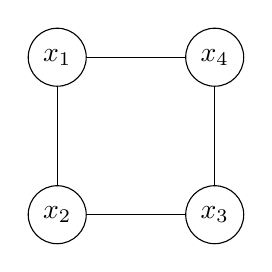
\begin{tikzpicture}[node distance=1.5cm, auto]

        % Nodes
        \node[circle, draw] (x1) at (0,2) {$x_1$};
        \node[circle, draw] (x2) at (0,0) {$x_2$};
        \node[circle, draw] (x3) at (2,0) {$x_3$};
        \node[circle, draw] (x4) at (2,2) {$x_4$};
        % \node[circle, draw] (x5) at (4,3) {$x_5$};
        
        % Edges
        \draw[-] (x1) -- (x4);
        % \draw[->] (x4) -- (x5);
        \draw[-] (x4) -- (x3);
        \draw[-] (x2) -- (x3);
        \draw[-] (x2) -- (x1);
        \draw[-] (x3) -- (x4);
        
        \end{tikzpicture}        
\end{minipage}


\section{Drawing an undirected graphical model}
There are majorly two ways to draw an undirected graphical model:

\begin{enumerate}
    \item {\bf Starting from factors:} We simply connect together all variables that appear together in a factor. Here are some real-life examples:
    \begin{itemize}
        \item Image pixels
        \begin{center}
        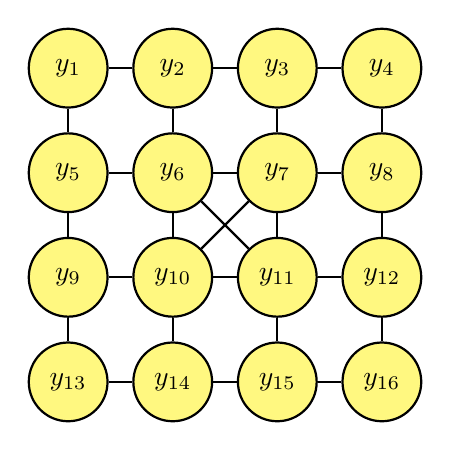
\begin{tikzpicture}[node distance=.3cm and .3cm, thick, every node/.style={circle, draw, fill=yellow!50, minimum size=1cm}]
            \node (y1) {$y_1$};
            \node[right=of y1] (y2) {$y_2$};
            \node[right=of y2] (y3) {$y_3$};
            \node[right=of y3] (y4) {$y_4$};
            \node[below=of y1] (y5) {$y_5$};
            \node[right=of y5] (y6) {$y_6$};
            \node[right=of y6] (y7) {$y_7$};
            \node[right=of y7] (y8) {$y_8$};
            \node[below=of y5] (y9) {$y_9$};
            \node[right=of y9] (y10) {$y_{10}$};
            \node[right=of y10] (y11) {$y_{11}$};
            \node[right=of y11] (y12) {$y_{12}$};
            \node[below=of y9] (y13) {$y_{13}$};
            \node[right=of y13] (y14) {$y_{14}$};
            \node[right=of y14] (y15) {$y_{15}$};
            \node[right=of y15] (y16) {$y_{16}$};
            \draw (y1) -- (y2);
            \draw (y2) -- (y3);
            \draw (y3) -- (y4);
            \draw (y1) -- (y5);
            \draw (y5) -- (y6);
            \draw (y6) -- (y7);
            \draw (y7) -- (y8);
            \draw (y5) -- (y9);
            \draw (y9) -- (y10);
            \draw (y10) -- (y11);
            \draw (y11) -- (y12);
            \draw (y9) -- (y13);
            \draw (y13) -- (y14);
            \draw (y14) -- (y15);
            \draw (y15) -- (y16);
            \draw (y2) -- (y6);
            \draw (y6) -- (y10);
            \draw (y6) -- (y11); 
            \draw (y7) -- (y10);
            \draw (y10) -- (y14);
            \draw (y11) -- (y15);
            \draw (y7) -- (y11);
            \draw (y3) -- (y7);
            \draw (y4) -- (y8);
            \draw (y8) -- (y12);
            \draw (y12) -- (y16);
        \end{tikzpicture}
    \end{center}

        \item Language Models from n-gram scores
        
        % \begin{center}
            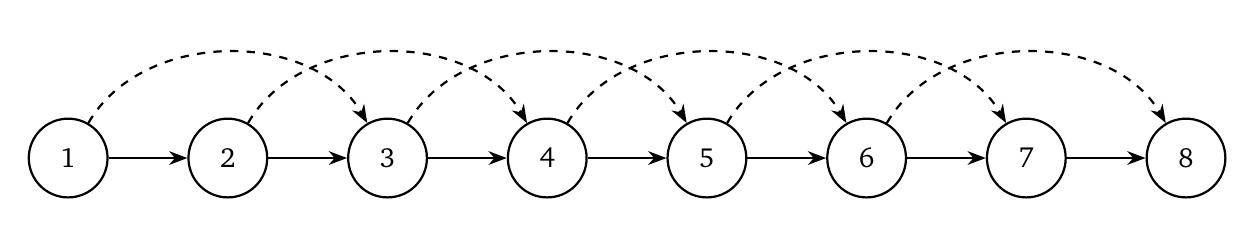
\begin{tikzpicture}[
                node/.style={circle, draw, thick, minimum size=1cm},
                edge/.style={-{Stealth}, thick},
            ]
            
            % Nodes in a linear arrangement
            \node[node] (n1) {1};
            \node[node, right=1cm of n1] (n2) {2};
            \node[node, right=1cm of n2] (n3) {3};
            \node[node, right=1cm of n3] (n4) {4};
            \node[node, right=1cm of n4] (n5) {5};
            \node[node, right=1cm of n5] (n6) {6};
            \node[node, right=1cm of n6] (n7) {7};
            \node[node, right=1cm of n7] (n8) {8};
            
            % Linear connections
            \draw[edge] (n1) -- (n2);
            \draw[edge] (n2) -- (n3);
            \draw[edge] (n3) -- (n4);
            \draw[edge] (n4) -- (n5);
            \draw[edge] (n5) -- (n6);
            \draw[edge] (n6) -- (n7);
            \draw[edge] (n7) -- (n8);
            
            % Additional connections
            \draw[edge, dashed] (n1) to[out=60, in=120] (n3);
            \draw[edge, dashed] (n2) to[out=60, in=120] (n4);
            \draw[edge, dashed] (n3) to[out=60, in=120] (n5);
            \draw[edge, dashed] (n4) to[out=60, in=120] (n6);
            \draw[edge, dashed] (n5) to[out=60, in=120] (n7);
            \draw[edge, dashed] (n6) to[out=60, in=120] (n8);
    
            \end{tikzpicture}
            
        % \end{center}
        The figure above illustrates a 3-gram model, where nodes separated by a distance of 2 are connected. This ensures that contiguous groups of three words are linked, allowing the model to capture the context and meaning within each phrase.
    \end{itemize}
    \item {\bf Starting from CIs }
\end{enumerate}



\section{Constructing an UGM from a positive distribution}
Positive distribution is a distribution where all the probabilities are non-negative. We are given $P(x_1, \dots, x_n)$ to which we can ask any CI of the form $X \perp\!\!\!\perp Y | Z$ and get a yes, no answer. 

Our goal is to draw a minimal, correct UGM $G$ to represent $P$. Here are the two options which we have ($V$ denotes the set of all $n$ variables):

\begin{itemize}
    \item {\bf Using pairwise CI:} For each pair of vertices $x_i, x_j $, if $x_i \not\perp\!\!\!\perp x_j | V - \{x_i, x_j\}$ in $P$, we add an edge between $x_i$ and $x_j$ in $G$. This is because for a UGM, the following is true:
    \[X \perp\!\!\!\perp Y | Z \implies X \perp\!\!\!\perp Y | Z, W\]
    The above might not be true for a bayesian network. It is true for a UGM because even after adding nodes to $Z$, $X$ and $Y$ will still be disconnected in the graph. Hence considering the entire set $V - \{x_i, x_j\}$ will also work.
    \item {\bf Using local CI:} For each node $x_i$, we need to find the smallest subset $U$ such that $x_i \perp\!\!\!\perp V - U - \{x_i\} | U$ in $P$. After this, we make the nodes in $U$, the neighbours of $x_i$ in $G$. 
\end{itemize}


\subsection{Example}
We are given the positive distribution $P(x, y, z, w)$ for which the following CIs hold:
\begin{itemize}
    \item $x \perp\!\!\!\perp y | z, w$
    \item $z \perp\!\!\!\perp w | x, y$
\end{itemize}


Let us first apply pairwise-CI algorithm to draw the graph $G$. We need to iterate over all the pairs of variables and check if the CI holds. If it does not hold, we add an edge between the two variables. So, for the edge $x, y$, they are independent given the other two variables ($x \perp\!\!\!\perp y | z, w$), so we do not add an edge. Similarly, for the edge $z, w$, they are independent given the other two variables ($z \perp\!\!\!\perp w | x, y$), so we do not add an edge. For all other edges, we add an edge (because the CI does not hold). So, the graph $G$ will look like this:

\begin{center}
    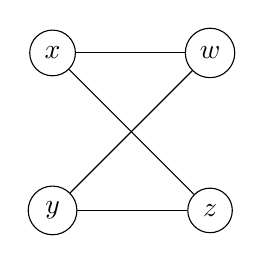
\begin{tikzpicture}[node distance=1cm, auto]
        \node[circle, draw] (x) at (0,2) {$x$};
        \node[circle, draw] (y) at (0,0) {$y$};
        \node[circle, draw] (z) at (2,0) {$z$};
        \node[circle, draw] (w) at (2,2) {$w$};
        \draw[-] (x) -- (z);
        \draw[-] (x) -- (w);
        \draw[-] (y) -- (z);
        \draw[-] (y) -- (w);
        \end{tikzpicture}
\end{center}

Now, let us try the same problem with the local-CI algorithm. We need to find $U$ for each of the four nodes. For $x$, $U$ is $\{z, w\}$ because $x \perp\!\!\!\perp V - U - \{x\} | U$ holds. For $y$, $U$ is $\{z, w\}$, for $z$, $U$ is $\{x, y\}$, for $w$, $U$ is $\{x, y\}$. We need to connect each node to the nodes in $U$. So, we will get the same graph as above.

\subsection{Markov Blanket}
UGMs are also called Markov Random Fields. 

The Markov Blanket of a variable $x_i$, $MB(x_i)$ is the smallest subset of variables $V$ that makes $x_i$ CI of others given the Markov Blanket. This is essentially the $U$, which we used above. 

\[x_i \perp\!\!\!\perp V - MB(x_i) - \{x_i\} | MB(x_i) \]


Also, one of the theorems says that $MB(x_i)$ is always unique for a positive distribution. The proof of this, has been left as a self-reading exercise (given in the slides).

\subsection{Hammersly Clifford Theorem}
If a positive distribution $P(x_1, \dots, x_n)$ conforms to the pairwise CIs of a UDGM $G$, then it can be factorized as per the cliques of $G$. This is the Hammersly Clifford Theorem. 

\[
P(x_1, \dots, x_n) \propto \prod_{C \in \mathcal{C}} \psi_C(y_C)
\]
The proof of this theorem has been left as an exercise for the reader (Theorem 4.8 of the KF book).


\section{Summary}
Let $P$ be a distribution and $H$ be an undirected graph of the same set of nodes. 

$Factorize(P, H) \implies Global-CI(P, H) \implies Local-CI(P, H) \implies Pairwise-CI(P, H)$

But only for positive distributions, we have the following:

$Pairwise-CI(P, H) \implies Factorize(P, H)$


% sharvanee's part


\section{Which MRFs have perfect BNs}
\subsection{Chordal or Triangulated Graphs}
A graph is chordal if it has no minimal cycle of length $\geq 4$.\\~\\
Here a minimal cycle is a cycle without a shortcut i.e, it is a cycle $x_1, x_2 \dots x_n, x_1$ such that there is no edge connecting any of the cycle's vertices apart from the edges that make up the cycle.
\\~\\
Consider the following examples
\\~\\
\begin{minipage}{0.45\textwidth}
    \centering
    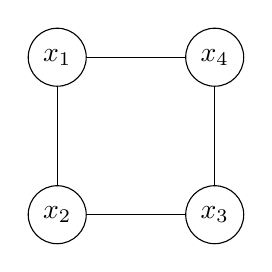
\begin{tikzpicture}[node distance=1.5cm, auto]
        % Nodes
        \node[circle, draw] (x1) at (0,2) {$x_1$};
        \node[circle, draw] (x2) at (0,0) {$x_2$};
        \node[circle, draw] (x3) at (2,0) {$x_3$};
        \node[circle, draw] (x4) at (2,2) {$x_4$};
        
        % Edges
        \draw[-] (x1) -- (x4);
        \draw[-] (x4) -- (x3);
        \draw[-] (x2) -- (x3);
        \draw[-] (x2) -- (x1);
        \draw[-] (x3) -- (x4);
    \end{tikzpicture}
    \captionof*{figure}{Not a chordal graph, since it contains a minimal cycle of length 4.}
\end{minipage}
\hfill
\begin{minipage}{0.45\textwidth}
    \centering
    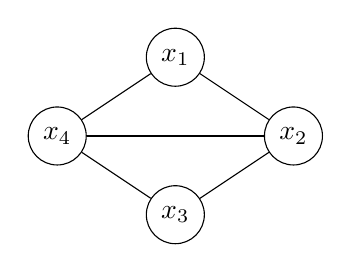
\begin{tikzpicture}[node distance=1.5cm, auto]
        % Nodes
        \node[circle, draw] (x1) at (0.5,2) {$x_1$};
        \node[circle, draw] (x2) at (2,1) {$x_2$};
        \node[circle, draw] (x3) at (0.5,0) {$x_3$};
        \node[circle, draw] (x4) at (-1,1) {$x_4$};
        
        % Edges
        \draw[-] (x1) -- (x2);
        \draw[-] (x2) -- (x3);
        \draw[-] (x3) -- (x4);
        \draw[-] (x4) -- (x1);
        \draw[-] (x2) -- (x4);
    \end{tikzpicture}
    \captionof*{figure}{Chordal graph, since it contains minimal cycles of only length 3. $x_1-x_2-x_3-x_4-x_1$ is not a minimal cycle because there is a shortcut between $x_2-x_4$.}
\end{minipage}

\vspace{1cm} % Space between rows of subfigures
\noindent
\begin{minipage}{0.45\textwidth}
    \centering
    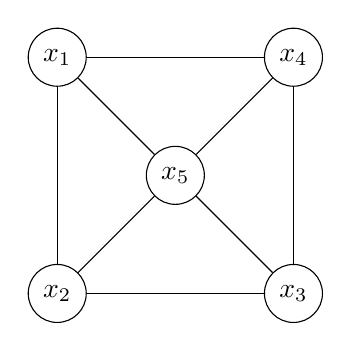
\begin{tikzpicture}[node distance=1.5cm, auto]
        % Nodes
        \node[circle, draw] (x1) at (0,3) {$x_1$};
        \node[circle, draw] (x2) at (0,0) {$x_2$};
        \node[circle, draw] (x3) at (3,0) {$x_3$};
        \node[circle, draw] (x4) at (3,3) {$x_4$};
        \node[circle, draw] (x5) at (1.5,1.5) {$x_5$};
        
        % Edges
        \draw[-] (x1) -- (x4);
        \draw[-] (x4) -- (x3);
        \draw[-] (x2) -- (x3);
        \draw[-] (x2) -- (x1);
        \draw[-] (x3) -- (x4);
        \draw[-] (x3) -- (x5);
        \draw[-] (x4) -- (x5);
        \draw[-] (x2) -- (x5);
        \draw[-] (x1) -- (x5);
    \end{tikzpicture}
    \captionof*{figure}{Not a chordal graph, since it contains a minimal cycle of length 4 ($x_1-x_2-x_3-x_4-x_1$). The paths via $x_5$ are not shortcuts because they consist of more than a single edge.}
\end{minipage}
\hfill
\begin{minipage}{0.45\textwidth}
    \centering
    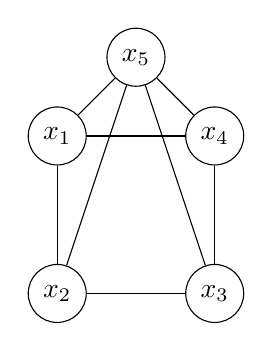
\begin{tikzpicture}[node distance=1.5cm, auto]
    % Nodes
    \node[circle, draw] (x1) at (0,2) {$x_1$};
    \node[circle, draw] (x2) at (0,0) {$x_2$};
    \node[circle, draw] (x3) at (2,0) {$x_3$};
    \node[circle, draw] (x4) at (2,2) {$x_4$};
    \node[circle, draw] (x5) at (1,3) {$x_5$}; % Elevated node on a different plane
    
    % Edges for the base (triangular graph)
    \draw[-] (x1) -- (x4);
    \draw[-] (x4) -- (x3);
    \draw[-] (x3) -- (x2);
    \draw[-] (x2) -- (x1);
    \draw[-] (x3) -- (x4);
    
    % Edges connecting the elevated node x5
    \draw[-] (x5) -- (x1);
    \draw[-] (x5) -- (x2);
    \draw[-] (x5) -- (x3);
    \draw[-] (x5) -- (x4);
\end{tikzpicture}

    \captionof*{figure}{The same graph as the one on the left, drawn for better visualization. Now we clearly see that the 4-cycle is minimal and doesn't contain a shortcut.}
\end{minipage}
\subsection{Perfect conversion of MRF to BN}
Theorem: An MRF can be converted perfectly into a BN iff it is chordal.\\~\\
(The proof of this theorem is left as an exercise using theorems 4.11 and 4.13 of the KF book).\\~\\ This conversion can be done using the PC algorithm since we know the BN is perfectly constructed.
\subsection*{Chordal Graphs}
Theorem: Every triangulated graph is either complete or has atleast two non-adjacent simplicial vertices. A vertex is simplicial if its neighbours form a complete graph.


\begin{minipage}{0.30\textwidth}
    \centering
    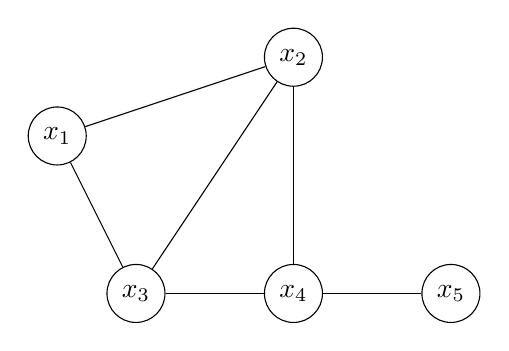
\begin{tikzpicture}[node distance=1.5cm, auto]

        % Nodes
        \node[circle, draw] (x1) at (-1,2) {$x_1$};
        \node[circle, draw] (x2) at (0,0) {$x_3$};
        \node[circle, draw] (x3) at (2,0) {$x_4$};
        \node[circle, draw] (x4) at (2,3) {$x_2$};
        \node[circle, draw] (x5) at (4,0) {$x_5$};
        
        % Edges
        \draw[-] (x1) -- (x4);
        \draw[-] (x3) -- (x5);
        \draw[-] (x4) -- (x3);
        \draw[-] (x2) -- (x3);
        \draw[-] (x2) -- (x1);
        \draw[-] (x3) -- (x4);
        \draw[-] (x2) -- (x4);
        
    \end{tikzpicture}        
\end{minipage}
\hfill
\begin{minipage}{0.60\textwidth}
    In the graph on the left, $x_1$ and $x_5$ are simplicial vertices. To see this, consider the neighbours of $x_1$ i.e., $\{x_2, x_3\}$. These vertices form a complete $K2$ graph, so $x_1$ is simplicial. $x_5$ has only one neighbour, $x_4$, which trivially forms a complete graph, making $x_5$ also simplicial. The other 3 vertices are not simplicial; this can be checked using their neighbour sets.
\end{minipage}\\~\\
The proof of this theorem is out of the scope of the course and can be found online.
\subsection{Algorithm to convert UGM to BN}
\begin{algorithm}
\caption{Conversion of UGM to BN}\label{alg:template}
\begin{algorithmic}[1]
    \STATE \textbf{Input:} Undirected graph $H$ with $n$ nodes
    \STATE \textbf{Output:} Directed graph $G$ over the same $n$ nodes
    % \STATE Initialize variables
    \FOR{$i:1\xrightarrow{}n$}
        \STATE $x_i\xleftarrow{}$ a simplicial node in $H$
        \STATE Remove $x_i$ and its associated edges from $H$. $H$ is now a reduced triangulated graph.
    \ENDFOR
    \STATE We now have the ordering $x_1, x_2 \dots x_n$
    \STATE Initialize empty graph $G \xleftarrow{} \phi$
    \FOR{$i:n\xrightarrow{}1$}
        \STATE Add node $x_i$ to $G$
        \STATE Draw an edge from $x_j$ to $x_i$ if $x_j$ is connected to $x_i$ in $H$ and $j>i$
    \ENDFOR
    \STATE \textbf{return} $G$
\end{algorithmic}
\end{algorithm}
Consider the following example to illustrate how the algorithm works

\begin{center}
    
    \begin{tikzpicture}
        \begin{tikzpicture}[node distance=1.5cm, auto]

            \node[circle, draw] (x1) at (2.5,3.5) {$1$};
            \node[circle, draw] (x2) at (4,2) {$3$};
            \node[circle, draw] (x3) at (2.5,0.5) {$4$};
            \node[circle, draw] (x4) at (1,2) {$2$};
            \node[circle, draw] (x5) at (6,2) {$5$};
            
            % Edges
            \draw[-] (x1) -- (x2);
            \draw[-] (x2) -- (x3);
            \draw[-] (x3) -- (x4);
            \draw[-] (x4) -- (x1);
            \draw[-] (x2) -- (x4);
            \draw[-] (x2) -- (x5);
            
        \end{tikzpicture}
    \end{tikzpicture}
\end{center}
% \vspace{1cm}
Following the steps of the algorithm, we remove the simplicial vertices one by one, in the order $4, 5, 1, 2, 3$ and $H$ is transformed as shown below.


\begin{figure}[h!]
    \centering
    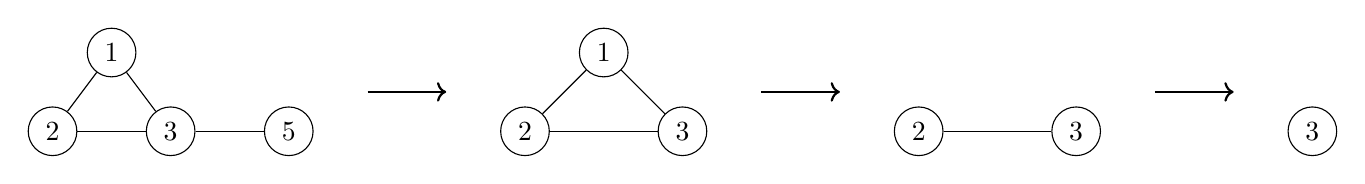
\begin{tikzpicture}[node distance=1.5cm, auto]

        % Nodes for the first plot
        \node[circle, draw] (x1) at (1.75, 3) {$1$};
        \node[circle, draw] (x2) at (2.5, 2) {$3$};
        \node[circle, draw] (x4) at (1, 2) {$2$};
        \node[circle, draw] (x5) at (4, 2) {$5$};
        
        % Edges for the first plot
        \draw[-] (x1) -- (x2);
        \draw[-] (x4) -- (x1);
        \draw[-] (x2) -- (x4);
        \draw[-] (x2) -- (x5);

        % Nodes for the second plot (increased horizontal distance)
        \node[circle, draw] (y1) at (8, 3) {$1$};
        \node[circle, draw] (y2) at (9, 2) {$3$};
        \node[circle, draw] (y4) at (7, 2) {$2$};
        
        % Edges for the second plot
        \draw[-] (y1) -- (y2);
        \draw[-] (y4) -- (y1);
        \draw[-] (y2) -- (y4);

        % Nodes for the third plot (further horizontal distance)
        \node[circle, draw] (z2) at (14, 2) {$3$};
        \node[circle, draw] (z4) at (12, 2) {$2$};
        
        % Edges for the third plot
        \draw[-] (z2) -- (z4);

        % Node for the fourth plot
        \node[circle, draw] (w2) at (17, 2) {$3$};

        % Horizontal arrows between the plots
        \draw[->, thick] (5, 2.5) -- (6, 2.5);  % Arrow between first and second plot
        \draw[->, thick] (10, 2.5) -- (11, 2.5);  % Arrow between second and third plot
        \draw[->, thick] (15, 2.5) -- (16, 2.5);  % Arrow between third and fourth plot

    \end{tikzpicture}
\end{figure}
Now starting from an empty graph $G$, we add the nodes in the order $3, 2, 1, 5, 4$ as per the algorithm.
\clearpage

\begin{figure}[h!]
    \centering
    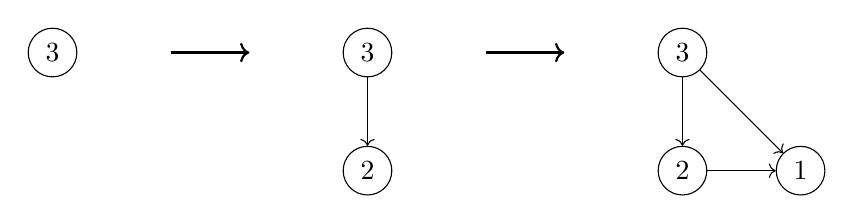
\begin{tikzpicture}[node distance=1.5cm, auto]

        % First sub-picture
        \node[circle, draw] (a1) at (0, 1.5) {$3$};

        % Arrow to second sub-picture
        \draw[->, thick] (1.5, 1.5) -- (2.5, 1.5);

        % Second sub-picture
        \node[circle, draw] (b1) at (4, 1.5) {$3$};
        \node[circle, draw] (b2) at (4, 0) {$2$};
        \draw[->] (b1) -- (b2);

        % Arrow to third sub-picture
        \draw[->, thick] (5.5, 1.5) -- (6.5, 1.5);

        % Third sub-picture
        \node[circle, draw] (c1) at (8, 1.5) {$3$};
        \node[circle, draw] (c2) at (8, 0) {$2$};
        \node[circle, draw] (c3) at (9.5, 0) {$1$};
        \draw[->] (c1) -- (c2);
        \draw[->] (c2) -- (c3);
        \draw[->] (c1) -- (c3);

    \end{tikzpicture}
\end{figure}


\begin{figure}[htp]
    \centering
    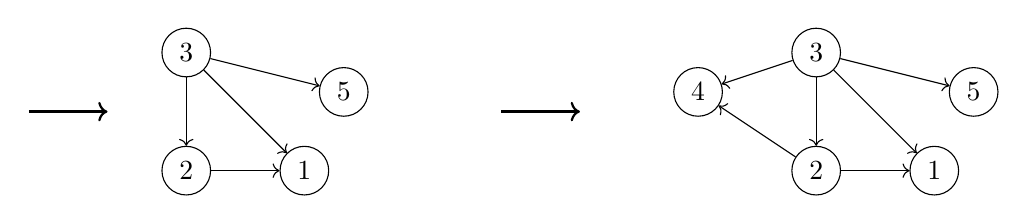
\begin{tikzpicture}[node distance=1.5cm, auto]

        % First diagram
        \node[circle, draw] (a1) at (0, 1.5) {$3$};
        \node[circle, draw] (a2) at (0, 0) {$2$};
        \node[circle, draw] (a3) at (1.5, 0) {$1$};
        \node[circle, draw] (a4) at (2, 1) {$5$};
        \draw[->] (a1) -- (a2);
        \draw[->] (a1) -- (a3);
        \draw[->] (a2) -- (a3);
        \draw[->] (a1) -- (a4);

        % Arrow from left to the first diagram
        \draw[->, thick] (-2, 0.75) -- (-1, 0.75);

        % Arrow between diagrams
        \draw[->, thick] (4, 0.75) -- (5, 0.75);

        % Second diagram
        \node[circle, draw] (b1) at (8, 1.5) {$3$};
        \node[circle, draw] (b2) at (8, 0) {$2$};
        \node[circle, draw] (b3) at (9.5, 0) {$1$};
        \node[circle, draw] (b4) at (10, 1) {$5$};
        \node[circle, draw] (b5) at (6.5, 1) {$4$};
        \draw[->] (b1) -- (b2);
        \draw[->] (b1) -- (b3);
        \draw[->] (b2) -- (b3);
        \draw[->] (b2) -- (b5);
        \draw[->] (b1) -- (b5);
        \draw[->] (b1) -- (b4);

    \end{tikzpicture}
\end{figure}
The final graph $G$ we obtain above is a perfect Bayesian Network representation of the undirected graph $H$. It has no immoralities (if it did, it could not be converted back to UGM without loss of information). Since the construction is perfect, we can go back and forth between BN and UGM while maintaining the set of CIs.

\end{document}
